\chapter{Related work}
\label{CapDA}

Absolventul va prezenta clar partea aplicativ? a lucr?rii ?i metodologia de solu?ionare folosind elementele teoretice.

Se va specifica mediul de lucru, a facilit??ilor folosite ?n acest mediu, proiectarea aplica?iei, detalii de implementare, exemple de test sau rezultate sub forma unor studii de caz, modul de utilizare a programului 
prin prezentarea documenta?iei de utilizare. Va fi anexat ?n lucrare inclusive codul surs?.

Partea dezvolt?rii aplicative poate fi constituit? din mai multe capitole.

Referirea unei figuri \ref{Cap3Figura3-1}.

\begin{figure}[htbp]
	\centering
		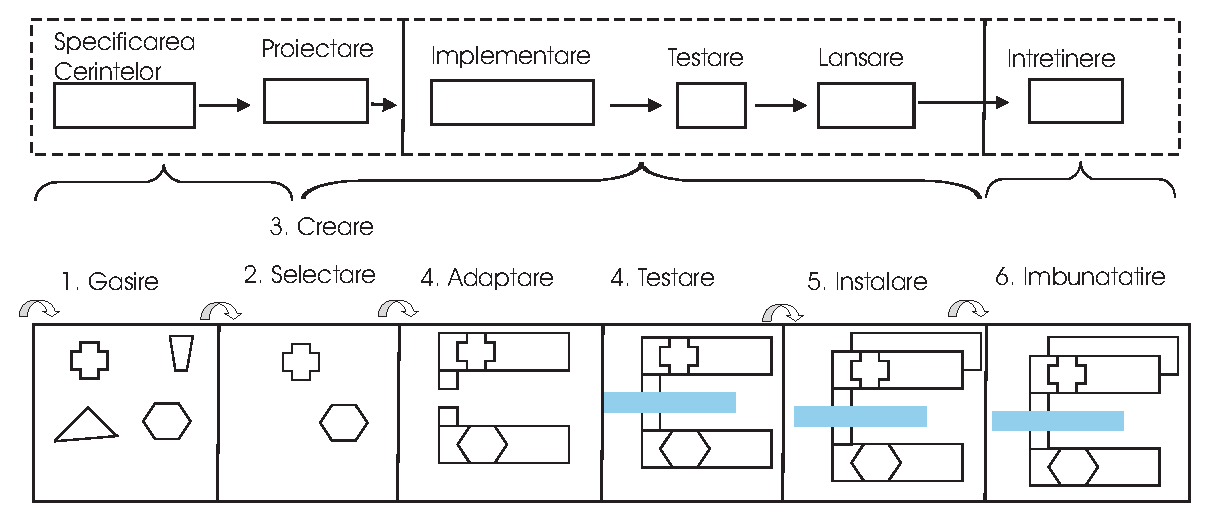
\includegraphics[scale=0.65]{Fig/fig_3_1.eps}
	\caption{Ciclul de dezvoltare al sistemelor bazate pe componente adaptat modelului cascad?}
	\label{Cap3Figura3-1}
\end{figure}


Referirea la Tabelul \ref{Cap3Tabel01}. 

\begin{table}[htbp]
\begin{center}
\begin{tabular}
{||p{100pt}||p{60pt}|p{60pt}||}
\hline
 Nume algoritm& 
 Toate solu?iile &
 Solu?ia optim?\\
\hline 
\hline Nume 1 & $20$ & $5$  \\
\hline Nume 2 & $20$ & $2$  \\
\hline
\end{tabular}
\end{center}
\caption{Solu?ii ob?inute }
\label{Cap3Tabel01}
\end{table}



